% ----------------------------------------------------------
% Teste test5_2_e50b128class2_20231212_030449
% ----------------------------------------------------------
\subsubsection{Teste test5_2_e50b128class2_20231212_030449 - AlexNet (Is That a Santa)}

Informações utilizadas para o treinamento.

\begin{table}[ht]
   \centering
   \caption{Treinamento}
   \label{tab:modelos}
   \begin{tabular}{| c | c | }
      \hline 
      \textbf{Informação} & \textbf{Descrição} \\
      \hline \hline 
      Rede & AlexNet \\
      \hline
      Número de épocas & 50\\
      \hline
      Tamanho do lote & 128\\
      \hline
      Taxa inicial & 0.01 \\
      \hline
      Taxa de decaimento & 0.0005 \\
      \hline
      Total de classes & 2\\
      \hline
      Dataset & CIFAR-10\\
      \hline
   \end{tabular} 
\end{table}

Resultados obtidos após treinamento.

\begin{tabular}{lrrrr}
\toprule
  Unnamed: 0 &  precision &   recall &  f1-score &    support \\
\midrule
       Santa &   0.979866 & 0.951140 &  0.965289 & 307.000000 \\
   Not Santa &   0.952532 & 0.980456 &  0.966292 & 307.000000 \\
    accuracy &   0.965798 & 0.965798 &  0.965798 &   0.965798 \\
   macro avg &   0.966199 & 0.965798 &  0.965791 & 614.000000 \\
weighted avg &   0.966199 & 0.965798 &  0.965791 & 614.000000 \\
\bottomrule
\end{tabular}


\begin{figure}[ht]
 \begin{center}
   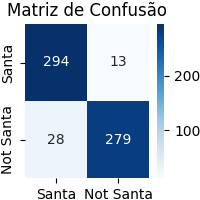
\includegraphics[scale=1]{tests/test5_2_e50b128class2_20231212_030449/confusion_matrix.png}
  \caption{Matriz de Confusão}
  \label{fig:fig03}
 \end{center}
\end{figure}

\begin{figure}[ht]
 \begin{center}
   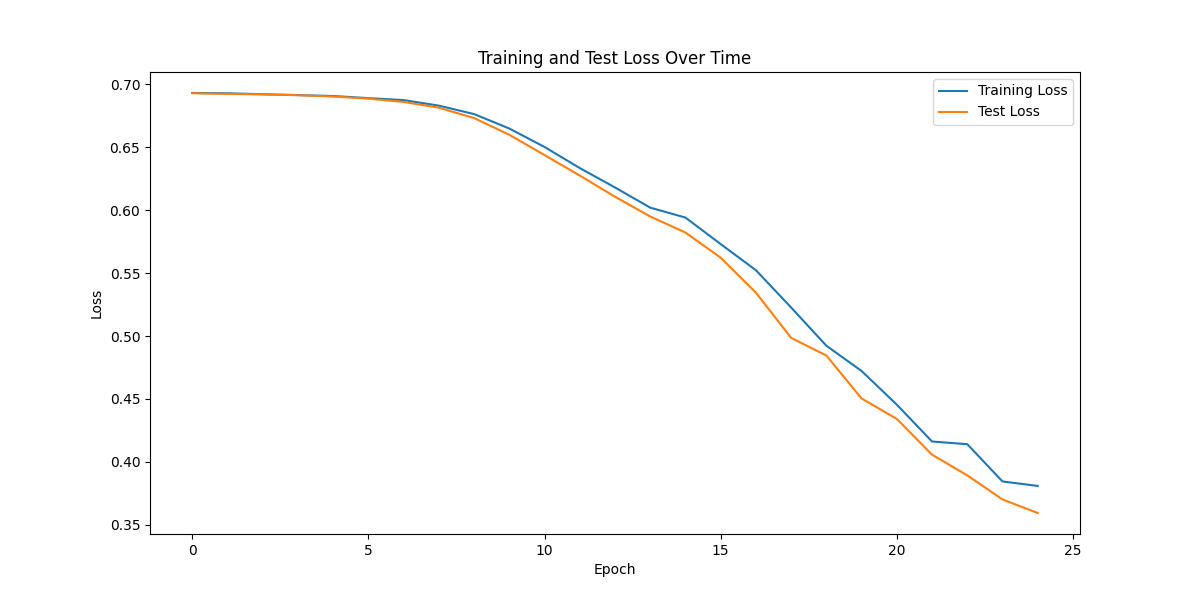
\includegraphics[scale=0.8]{tests/test5_2_e50b128class2_20231212_030449/loss_over_time.png}
  \caption{Gráfico de Perda}
  \label{fig:fig04}
 \end{center}
\end{figure}
